% new tcolorbox environment
%\newtcolorbox{topQuark}[2][]{
%  coltext      = black,
%  colframe     = \MyBlockFrameColorLeft,
%  colback      = \MyBlockFillColorLeft,
%  colbacktitle = \MyBlockTitleBoxColor,
%  coltitle     = black,
%  title        = {\Large{\textbf{#2}}},
%  fonttitle    = \bfseries,
%  boxrule      = 0.2cm, %frame line width
%  %tikz={rotate=#3}, % manipulate the tcolorbox as a whole (in degrees)
%  top=+0.0cm, bottom=+0.0cm, left=+0.05cm, right=+0.05cm,
%  %enlarge top by   = +1.0cm,  %  equivalent to mdframed 'skipabove'
%  %enlarge bottom by= +0.0cm,  %  equivalent to mdframed 'skipbelow'
%  %enlarge left by  = +1.5cm,  
%  %enlarge right by = +0.0cm, 
%  opacityback=1.0, % 1.0 means totally transparent, 0.0 means totally opaque
%  arc=0.0cm,        % 0.0cm for non-rounded corners!
%  #1,
%}

% CMS
\begin{topQuark}[enhanced, tikz={rotate=0}]{Multi-Muons In CDF: The Mystery Continues}
  %\begin{multicols}{2}
    We present a phenomenological conjecture of new physics that is suggested
    by the topology and kinematic properties of the multi-muon events recently
    reported by the CDF collaboration. We show that the salient features of 
    the data can be accounted for by postulating the pair production of
    three new states $h_1$, $h_2$, and $h_3$ with masses in the range
    of 15, 7.3, and 3.6 GeV/c$^{2}$, respectively. The heavier states 
    cascade-decay into the lighter ones, whereas the lightest state 
    decays into a $\tau$ pair with a lifetime of the order of 20 ps.
    \begin{comment}
    % ========================
    \begin{figure}
      \begin{center}
        \vspace{-0.2in}
        \leavevmode
        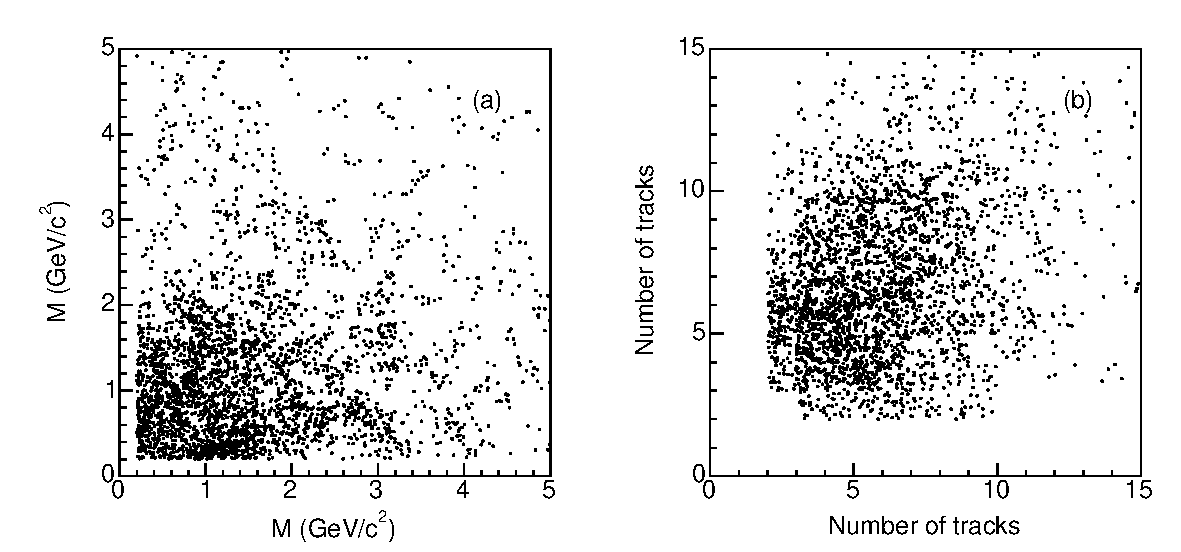
\includegraphics[width=\textwidth]{./figures/MultiMuons2_CDF.pdf}
        %\caption[]{Two-dimensional distributions, reproduced from Ref.~\cite{a0disc},
        %  of (a) the invariant mass, $M$, of all muons and (b) the total
        %  number of tracks contained in a $36.8^{\deg}$ cone when both
        %  cones contain at least two muons.}
      \end{center}
    \end{figure}
    % ========================
    \end{comment}
%  \end{multicols}
\end{topQuark}
